% SigDrop journal draft v2 (2026-11-26): forest scenario, front part (Introduction to Problem Formulation).
% Build: ./build.sh -> main.pdf. Sources of every number: ../README-vi.md.
\documentclass[journal,10pt]{IEEEtran}
\usepackage[T1]{fontenc}
\usepackage[utf8]{inputenc}
\usepackage{amsmath,amssymb,amsthm}
\usepackage{graphicx}
\usepackage{booktabs}
\usepackage{cite}
\usepackage{xcolor}
\usepackage{url}
\graphicspath{{../../figures/}{../../draft-v1/figs/}}
\newtheorem{theorem}{Theorem}
\newtheorem{proposition}{Proposition}
\theoremstyle{definition}
\newtheorem{definition}{Definition}
\newtheorem{assumption}{Assumption}
\theoremstyle{remark}
\newtheorem{remark}{Remark}
\newcommand{\todo}[1]{\textcolor{red}{[TODO: #1]}}
\newcommand{\open}[1]{\textcolor{blue}{[OPEN: #1]}}
\newcommand{\Tp}{T_{\mathrm p}}
\newcommand{\spine}{\textsc{Spine}}
\newcommand{\lmtour}{\textsc{LM-Tour}}
\newcommand{\chord}{\textsc{Chord}}
\newcommand{\river}{\textsc{River}}
\DeclareMathOperator*{\argmin}{arg\,min}

\begin{document}
\title{Finding a Missing Person with a Forest IoT Network: Single-Pass UAV Query Delivery with Planned Ground Cooperation}
\author{\todo{authors and affiliations}%
\thanks{Draft v2 of the journal version (2026-11-26), forest scenario; Sections I--V only. A preliminary version was
submitted to IEEE ICC 2027.}}
\maketitle

\begin{abstract}
When a person goes missing in a national park, the cameras and sensors already installed in the forest may have seen
them, but the forest core has no cellular coverage and its battery-powered devices are linked only by low-power radios.
We push a compact search query, a set of reference images of several hundred kilobytes, from the ranger station to the
few AI-capable devices, and let them report matches over LoRa. A fixed-wing UAV can broadcast the query over IEEE
802.15.4 in one pass, but under the canopy its air-to-ground range drops to 100--200\,m, so most AI nodes hear only a
fraction of the query. We split the mission into three phases: an offline phase that selects the AI cells and plans the
operation, a delivery phase in which one fixed-wing pass is completed by a ground transport planned from the flight
geometry, and a verification phase in which a rotary-wing UAV visits the cells that reported a match. The objective is
the 0.9-quantile of the time from take-off until the person is confirmed. We formulate the three phases as three
optimisation problems, a capacitated facility location problem with congestion constraints, a Dubins routing problem
with neighbourhoods coupled with a time-expanded unit-capacity flow, and a latency-type online routing problem, and we
place each in its known complexity class. \todo{results sentence once Sections VI--VIII are rewritten for the forest
scenario.}
\end{abstract}
\begin{IEEEkeywords}
UAV, search and rescue, forest wireless sensor networks, IEEE 802.15.4, cooperative dissemination, Dubins traveling
salesman problem, facility location, edge AI.
\end{IEEEkeywords}

\section{Introduction}\label{sec:intro}
Search and rescue (SAR) in protected areas is frequent and time-critical. The parks managed by the U.S. National Park
Service recorded 2\,890 SAR incidents in 2017, and an average of 11.2 per day over 1992--2007
\cite{heggie2009}\todo{verify both numbers on the full text; add a source for Vietnam}. Survival falls quickly with time:
among lost persons with dementia in Virginia, all of those found within 12\,h survived, whereas a third of those found
after 24\,h did not \cite{koester1998}. Searchers start from a last-seen point and expand outwards on foot, with dogs
and with aircraft; in a lowland tropical forest the canopy hides the ground from the air, and visual search from above
is of little use.

Meanwhile, forests are being instrumented. Camera traps are a standard tool of wildlife monitoring, and networked
camera traps now send images over 4G with solar power, e.g., 65 cameras on 34\,km$^2$ of a Natura~2000 site
\cite{kissling2024}. Wildfire sensors form LoRa meshes of about one node per hectare in pilot sites, and one vendor
reports more than 30\,000 deployed sensors \cite{dryad}; GreenOrbs ran up to 330 IEEE 802.15.4 nodes in a forest
\cite{liu2013greenorbs}. Some of these devices, or an edge box next to them, can run a person detector or a
re-identification network. A person lost in such a forest may thus have walked past a device that recorded them, but no
device knows whom to look for, and the forest core has no cellular coverage through which the footage could be
uploaded. We therefore push a compact query down to the devices instead of pulling footage up. Because different
vendors run different embedding models whose vectors are not comparable \cite{shen2020}, the query carries reference
images, $L=12$ images or about 400\,kB, so that each AI node embeds them with its own model.

\begin{figure}[t]\centering
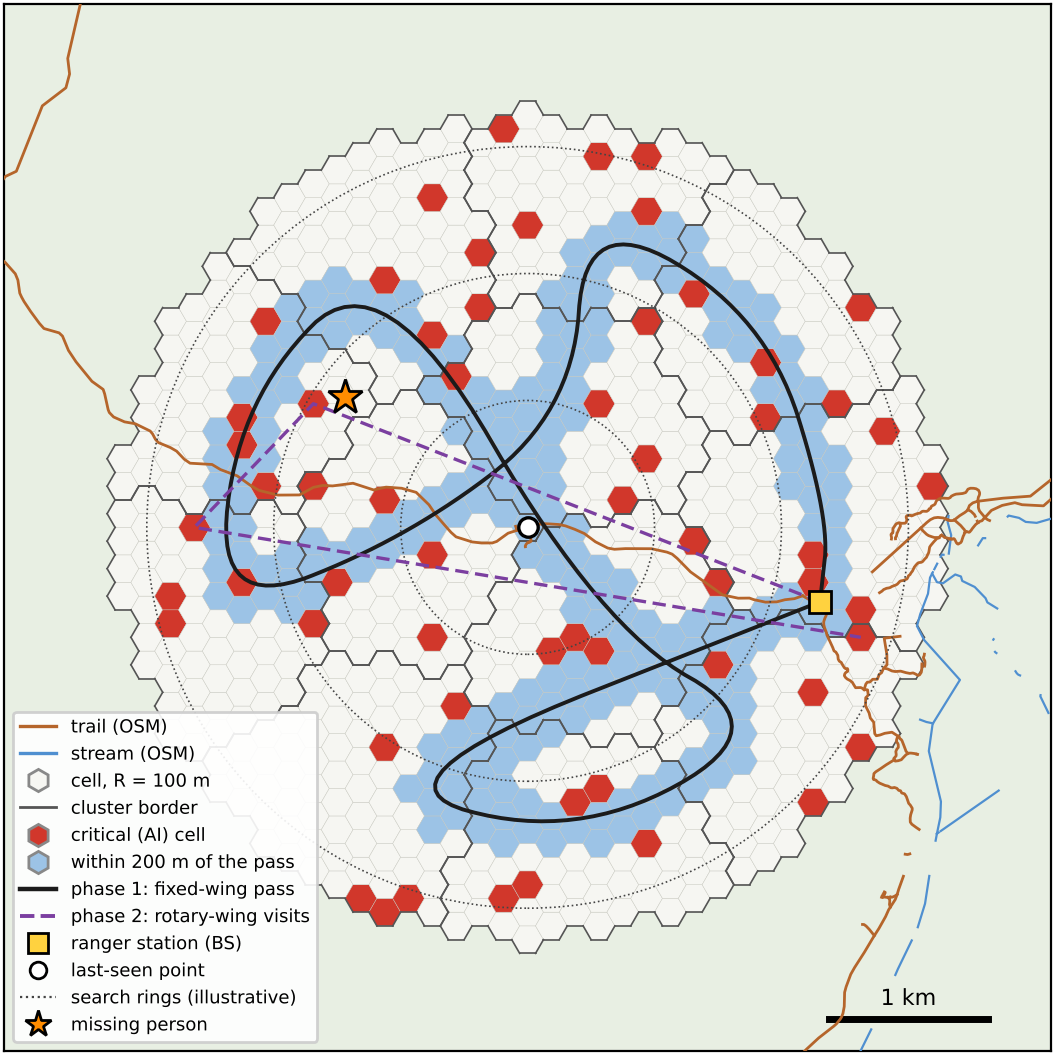
\includegraphics[width=\columnwidth]{draft2-scenario-cattien-labelled.png}
\caption{Scenario on a $6.6\times6.6$\,km window of Cat Tien National Park, Vietnam (trails and streams from
OpenStreetMap). The network around the last-seen point is tiled into cells of radius 100\,m grouped into 12 clusters;
60 cells host an AI node. One fixed-wing pass from the ranger station (phase~1) reaches the cells within about 200\,m
of its track; the ground network carries the query to the remaining AI cells. After the AI nodes report, a rotary-wing
UAV visits the suspected cells (phase~2). Clusters, AI cells, paths and rings are illustrative.}\label{fig:scenario}
\end{figure}

\textbf{Why existing means fall short.} The query cannot travel over LoRa: at spreading factor~7 under a 10\,\% duty
cycle, 400\,kB need at least 1.8\,h of airtime, and 18\,h under a 1\,\% duty cycle, even if every cluster head is in range
of the station. It cannot travel over the 802.15.4 mesh from the station either: the station sits at the forest edge,
the AI nodes are 50--95 radio hops away on our maps, and the measured rates of bulk dissemination protocols translate
into 20\,min to more than an hour at that depth \cite{liang2008,du2017}\todo{redo the hop count on the forest maps}. A
fixed-wing UAV can fly over the forest in minutes and broadcast the query, but it cannot hover and crosses each cluster
once. Under the canopy the air-to-ground (A2G) range of 802.15.4 drops to 100--200\,m (Section~\ref{sec:model}), so a
cell hears only the few hundred packets emitted while the UAV is overhead, and the AI nodes, which are rarely on the
track, cannot assemble the query alone. Making the UAV dwell above every AI node until it has decoded a rateless code
\cite{zeng2018multicast} costs airtime at every receiver: in our conference version we proved that every scheme in
which a device relies only on what its own cell hears from the UAV needs at least the query airtime multiplied by a
fractional covering number of the AI cells, which reaches 35--76 at 100\,m range on our maps (Fig.~\ref{fig:bound}).

\begin{figure}[t]\centering
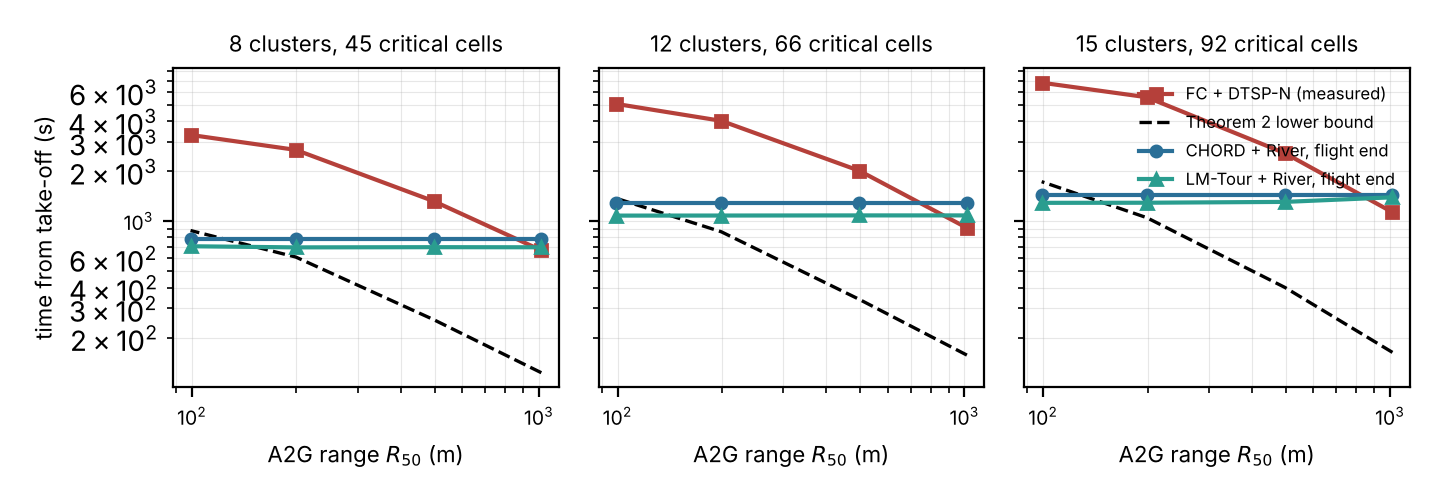
\includegraphics[width=\columnwidth]{bound-nc.png}
\caption{Why direct reception fails under the canopy. Time from take-off on three synthetic forest maps versus the A2G
range $R_{50}$. Red: fountain-coded loitering (FC + DTSP-N), measured in ns-3. Dashed: lower bound for every
non-cooperative scheme. Blue and green: the time at which the planned-cooperation flights end. \todo{redraw for the
forest maps with labels in the paper style.}}\label{fig:bound}
\end{figure}

\textbf{Key insight.} Packet $s$ of the broadcast is emitted at a point of a flight path that the base station designs.
Before take-off the station therefore knows which segment of the stream lands on which cell, and can plan the ground
cooperation that carries the missing segments to the AI nodes: the flight geometry is the transmission schedule.

\textbf{Three phases and their trade-offs.} We organise a mission into three phases (Fig.~\ref{fig:phases}). Phase~0
runs offline: the station selects the cells that host AI nodes and the assignment of the other devices to them, and
precomputes flight and ground plans. Phase~1 starts with the incident: a fixed-wing UAV broadcasts the query in one pass
and the ground network carries the missing parts to the AI cells, which match the query against their stored detections
and report over LoRa. Phase~2 sends a rotary-wing UAV to verify the suspected cells in an order driven by the posterior
probability of the person's location. The phases trade against each other. More AI cells shorten the paths of the
background data from the devices to their AI node, but give phase~1 more cells to serve and phase~2 more false alarms;
a flight that passes close to every AI cell is longer; and the order in which phase~1 serves the clusters decides when
phase~2 learns where to go.

\textbf{Objective.} We minimise the 0.9-quantile of the time $T^\star$ from take-off until the person is confirmed,
subject to the background-traffic budget, the hop limit and memory of the AI nodes, the energy of battery-powered
devices and the endurance of both UAVs. We report the mean as well.

\textbf{Contributions.} This paper extends our conference version \todo{cite ICC 2027 submission} as follows.
\begin{enumerate}
\item \emph{Scenario and model.} A model of query delivery in a lowland forest, with A2G and ground links attenuated by
foliage, battery-powered devices and a prior on the person's location (Sections~\ref{sec:system}--\ref{sec:model}). We
report the device densities of real forest deployments and state openly that our density is a forward-looking
assumption.
\item \emph{Formulation and complexity.} Three core problems, one per phase: (P0) a single-source capacitated facility
location problem with hop and congestion constraints; (P1) a Dubins traveling salesman problem with neighbourhoods
coupled with a time-expanded multicommodity flow on unit-capacity media; and (P2) an online latency-type routing
problem. (P1) is NP-hard already without ground links, and we identify the known hard problems that (P0) and (P2)
contain (Section~\ref{sec:problem}).
\item \emph{Limits.} \todo{Section VI: covering bound for non-cooperative delivery, single-radio and LP bounds for the
ground transport, restated for the forest model.}
\item \emph{Algorithms.} \todo{Section VII: AI-cell selection, \chord{}/\lmtour{}, load-balanced \river{} with shared
trees, takeover with adaptive radius, phase-2 policy.}
\item \emph{Evaluation.} \todo{Section VIII: ns-3 with a full 802.15.4 MAC on forest maps.}
\end{enumerate}

\begin{figure}[t]\centering
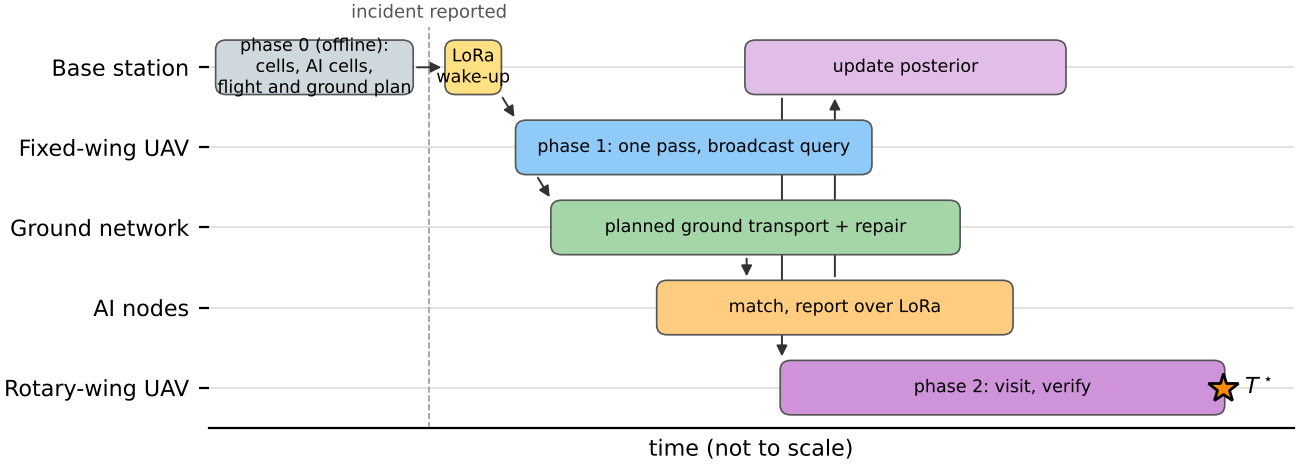
\includegraphics[width=\columnwidth]{draft2-phases-labelled.png}
\caption{Timeline of one mission. Phase~0 runs before any incident. Phase~1 overlaps the ground transport, the matching
and the LoRa reports; phase~2 can start as soon as the first report arrives. $T^\star$ is the time at which the person
is confirmed.}\label{fig:phases}
\end{figure}

\section{Related Work}\label{sec:related}
\textbf{UAV-enabled multicasting and data collection.} Trajectories are routinely optimised jointly with communication
\cite{zeng2016mag,mozaffari2019,wu2018}. Zeng \emph{et al.} \cite{zeng2018multicast} minimise the time for every ground
terminal to recover a common file directly from a rotary-wing UAV, and name a subsequent device-to-device sharing phase
as future work. Data collection from sensor networks, the reverse direction, jointly designs the wake-up schedule and
the trajectory \cite{zhan2018}, or clusters the sensors and plans multi-UAV tours under endurance constraints
\cite{nguyen2023gambac}. We consider a fixed-wing UAV that cannot dwell, receivers that are a known subset of a
multi-hop 802.15.4 mesh, and ground cooperation planned from the trajectory before take-off.

\textbf{Dissemination and routing in sensor networks.} Deluge \cite{hui2004} and Trickle \cite{levis2004} spread an
object by advertise--request epidemics; Typhoon \cite{liang2008}, Splash \cite{doddavenkatappa2013} and Pando
\cite{du2017} speed this up with channel switching, constructive interference and fountain codes. All of them start
from a sink and target every node. Minimum-latency broadcast scheduling \cite{you2013} asks for the shortest schedule
that informs all nodes under interference, with one source. Our transport differs in where the data enters (a known
segment at every cell under the track), in whom it targets (a few AI cells) and in that the plan follows from the
flight. Routing around holes with balanced load \cite{nguyen2021hole} is related to routing around cells without
devices, e.g., rivers and clearings.

\textbf{Forest networks and channels.} GreenOrbs \cite{liu2013greenorbs} measured a large 802.15.4 network in a
forest; networked camera traps \cite{kissling2024} and wildfire meshes \cite{dryad} are the deployments closest to ours.
Foliage loss at microwave frequencies is modelled empirically \cite{weissberger1982,itu833}; field tests of 2.4\,GHz
802.15.4 links from UAVs report ranges well below nominal and an altitude optimum near 45\,m \cite{nekrasov2019}.

\textbf{Curvature-constrained routing.} The Dubins TSP is NP-hard \cite{leny2012}; with neighbourhoods it is solved in
practice by sampling entry configurations and transforming the generalised TSP into an asymmetric TSP
\cite{isaacs2011,noon1993,obermeyer2009}. Our tours use these building blocks, but the objective is the readiness time
of the ground transport rather than tour length.

\textbf{Search theory and lost-person behaviour.} The optimal searcher path problem is NP-hard
\cite{trummel1986}; the minimum latency problem, its deterministic counterpart, is NP-hard even on weighted trees
\cite{sitters2002}; expanding search, where the searched region grows from a root, admits exact and approximation
algorithms \cite{hermans2019}. Lost-person statistics give the distance from the last-seen point by subject category
\cite{koester2008,koester1998}. We use these results to model the prior of phase~2 and to place (P2).

\section{System Operation}\label{sec:system}
This section describes one mission in words; Section~\ref{sec:model} gives the model and notation.

\textbf{Setting.} The protected area is a lowland forest with gentle relief, such as Cat Tien National Park in southern
Vietnam (Fig.~\ref{fig:scenario}). The park operator owns a network of battery-powered devices: camera traps that take
pictures on motion, acoustic and wildfire sensors, and a few AI nodes, i.e., smart cameras or edge boxes placed in
clearings where a solar panel can power a neural accelerator. The devices share an IEEE 802.15.4 mesh at 2.4\,GHz. A
cluster head (CH) in each cluster of cells also has a LoRa radio that reaches the ranger station. The ranger station at
the forest edge hosts the base station (BS), a LoRa gateway, and the take-off sites of two UAVs: a fixed-wing VTOL for
delivery (team~1) and a rotary-wing UAV with a camera for verification (team~2).

\textbf{Step 1: phase 0, offline.} Long before any incident, the BS
\begin{enumerate}
\item tiles the area into hexagonal cells, elects a cell leader (CL) in every cell and a gateway pair between adjacent
cells, and groups the cells into clusters;
\item selects the AI cells and assigns every ordinary device to one AI node within a hop limit, so that the background
data of the devices (crops or embeddings of the persons they detect) stay within the traffic and memory budgets;
\item precomputes, for a set of plausible incident areas, the flight plan of team~1 and the ground transport that
complements it, and distributes the per-cell part of the plan through the mesh.
\end{enumerate}
The selection is refreshed when devices fail or are added; the plans are cheap to recompute.

\textbf{Step 2: incident.} A person is reported missing, with a last-seen point and a description. The BS builds the
query from reference photographs supplied by relatives, fixes the incident area around the last-seen point, picks or
recomputes the plan, and broadcasts a LoRa wake-up message of a few bytes with the mission identifier and the take-off
time. From the plan, every device in the incident area computes when it must be awake.

\textbf{Step 3: phase 1, delivery.} Team~1 takes off and flies the planned pass at constant altitude, broadcasting the
query packets in a fixed order. Every cell under the track keeps what its devices hear. As soon as a cell holds the
segment it is planned to forward, it sends it towards the AI cells over the cell-level routes of the plan. A repair
step fills the gaps left by lost packets or by a track that deviates from the plan, e.g., because of wind. When an AI
node holds the complete query, it matches the query against its stored detections and those of its assigned devices,
and sends a score of a few bytes through its CH to the BS over LoRa.

\textbf{Step 4: phase 2, verification.} The BS turns the reports into a posterior over the cells. Team~2 takes off,
flies to the cell with the best ratio of posterior to travel time, verifies it with its own camera, and continues with
the next cell; the order is recomputed when new reports arrive. The mission ends when team~2 confirms the person; the
coordinates are passed to the ground team.

Two remarks on scope. First, a single UAV serves phase~1; several UAVs would need a coordination mechanism that we leave
for future work. Second, the scenario is restricted to flat or gently rolling forest, where the UAV can hold a constant
altitude and the ground can be treated as a plane. Mountain parks add terrain shadowing and terrain-following flight
(Section~\ref{sec:model}), which we treat as an extension.

\section{System Model}\label{sec:model}
Table~\ref{tab:notation} lists the main symbols. Assumptions used only in the analysis are numbered.

\begin{table}[t]\centering
\caption{Main notation}\label{tab:notation}
\footnotesize
\begin{tabular}{@{}ll@{}}
\toprule
Symbol & Meaning\\
\midrule
$G=(\mathcal C,\mathcal E)$ & cell graph; $\mathcal E$: pairs of adjacent cells (gateway pairs)\\
$\mathcal M$ & media: every cell and every gateway pair\\
$V$, $V_{\mathrm p}\subseteq V$ & devices; devices eligible as AI nodes\\
$K\subseteq\mathcal C$ & critical cells, i.e., cells hosting an AI node\\
$Q$, $\Tp$ & packets of the query; airtime of one UAV packet\\
$\tau_f$ & medium occupancy of one acknowledged ground hop\\
$q(t)$, $T_{\mathrm f}$ & track of team~1; flight duration\\
$P_c(x)$ & probability that cell $c$ hears a packet sent above $x$\\
$C_k$ & completion time of critical cell $k$\\
$E_u$ & energy budget of device $u$ for one mission\\
$\pi_c$ & prior probability that the person is in cell $c$\\
$c^\star$, $\omega$ & cell of the person; all other randomness\\
$T^\star$ & time from take-off until the person is confirmed\\
\bottomrule
\end{tabular}
\end{table}

\subsection{Area and terrain}
We surveyed $10\times10$\,km windows of eight protected areas with OpenStreetMap and a 25\,m elevation grid
(Table~\ref{tab:terrain}). They fall into two groups. In lowland or gently rolling forest the elevation varies by less
than 50\,m within 100\,m of a cell centre, small against the flight altitude of 100\,m. In mountain parks it varies by
90--160\,m (median) and up to 300\,m (90th percentile), more than the flight altitude, and more than half of the area
can be steeper than $30^\circ$. Our model treats the ground as a plane and therefore covers the first group; the second
needs terrain-following flight and terrain shadowing of both A2G and ground links.

\begin{assumption}[Flat ground]\label{as:flat}
Devices lie on a plane; the UAV flies at constant height $h$ above it.
\end{assumption}

\begin{table}[t]\centering
\caption{Terrain of four of the eight surveyed $10\times10$\,km windows}\label{tab:terrain}
\footnotesize
\begin{tabular}{@{}lrrrr@{}}
\toprule
Window & Elev.\ (m) & Slope & $>30^\circ$ & Relief (m)\\
\midrule
Cat Tien (VN) & 83--247 & $4^\circ$ & 0\,\% & 14 / 26\\
Bayerischer Wald (DE) & 764--1\,440 & $10^\circ$ & 0\,\% & 44 / 79\\
Bach Ma (VN) & 32--1\,455 & $28^\circ$ & 40\,\% & 126 / 185\\
Hoang Lien (VN) & 1\,180--3\,117 & $32^\circ$ & 58\,\% & 156 / 227\\
\bottomrule
\multicolumn{5}{@{}p{0.95\columnwidth}@{}}{\scriptsize Slope: median. $>30^\circ$: share of the area steeper than
$30^\circ$. Relief: elevation range within 100\,m of a cell centre, median / 90th percentile over the cells. The other
four windows (Cuc Phuong, Yosemite, Great Smoky Mountains, Kinabalu) belong to the mountain group.}
\end{tabular}
\end{table}

\subsection{Network, cells and devices}
The area is tiled by hexagonal cells of radius $R_{\mathrm c}=100$\,m. Every cell has a cell leader (CL); two adjacent
cells are joined by exactly one gateway pair; cell channels follow a 7-colour reuse and every gateway pair has its own
radio and channel. Let $G=(\mathcal C,\mathcal E)$ be the cell graph. Cells are grouped into clusters of at most 80
cells, each with a cluster head (CH) that has a LoRa uplink to the BS. Every cell and every gateway pair is one
\emph{medium} $m\in\mathcal M$: at most one of its radios transmits at a time.

The devices $V$ are camera traps, acoustic and wildfire sensors. A subset $V_{\mathrm p}\subseteq V$ can serve as AI
nodes: devices in a clearing with a solar panel and a neural accelerator, or an edge box next to them. A cell that hosts
an AI node is a \emph{critical cell}; $K$ denotes their set. Cells without devices (rivers, swamps) are holes of $G$.

\textbf{Density.} The cell graph is connected only if every cell has devices close enough to its neighbours. With an
urban street-canyon model of the ground links this requires devices at most about 50--60\,m apart, i.e., roughly 300
devices per km$^2$ \todo{redo for the foliage model of Section~\ref{sec:g2g}}. We use 816 devices per km$^2$ as in our
conference version. Real forest deployments are far sparser (Fig.~\ref{fig:density}): park-wide densities range from
0.003 to 2 devices per km$^2$, and only small pilot sites exceed 100. These sparse networks connect devices directly to
4G, LoRa or satellites, or not at all. Our density is therefore a forward-looking assumption, motivated by falling device
prices, by vendors that already deploy tens of thousands of forest sensors \cite{dryad}, and by the possibility of
sharing one mesh among camera, fire and acoustic networks. Section~\ref{sec:eval} reports the sensitivity to lower
densities. \todo{sensitivity to 400 and 280 devices per km$^2$.}

\begin{figure}[t]\centering
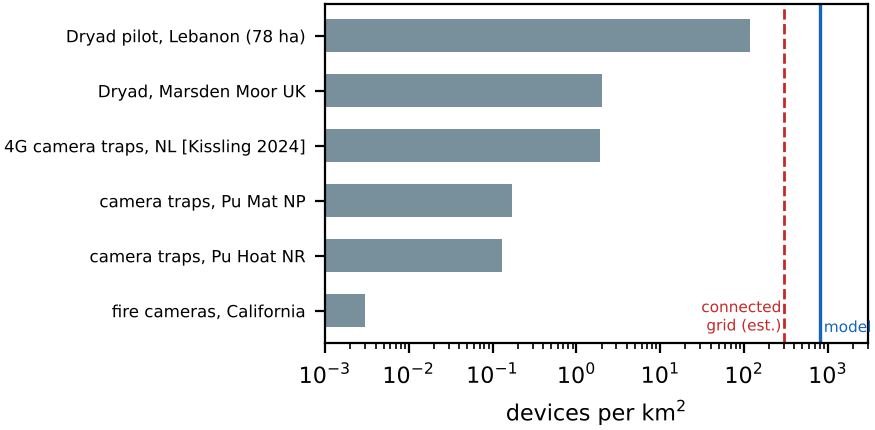
\includegraphics[width=\columnwidth]{draft2-density-gap-labelled.png}
\caption{Device density of real forest deployments (bars, log scale) against the density at which a cell grid of radius
100\,m stays connected (dashed, urban estimate) and the density of our model (solid). Densities are devices divided by
the area stated in each source.}\label{fig:density}
\end{figure}

\subsection{Energy and wake-up}\label{sec:energy}
All devices run on batteries, possibly with a small solar panel that is weak under the canopy. A device sleeps between
its own sensing events. Device $u$ has an energy budget $E_u$ for one mission; it spends $e_{\mathrm{rx}}$ per second
awake with its radio listening and $e_{\mathrm{tx}}$ per transmitted frame. When a mission starts, the BS broadcasts a
LoRa message with the mission identifier and the take-off time; from the plan, the devices of cell $c$ compute a wake
window $[t^{\mathrm{on}}_c,t^{\mathrm{off}}_c]$ that covers the UAV pass over $c$ and the ground transport through $c$.
\open{energy numbers of a camera trap and a sensor node; whether the CH stays awake.}

\subsection{UAVs and emission}
Team~1 is a fixed-wing VTOL at height $h=100$\,m with speed $v\in[25,50]$\,m/s and bank angle at most $45^\circ$, hence a
turning radius $\rho(v)=v^2/g$: 255\,m at 50\,m/s and 63.7\,m at 25\,m/s. It broadcasts one packet of 99\,B payload every
$\Tp=10$\,ms. Its track is a curve $q:[0,T_{\mathrm f}]\to\mathbb R^2$ from and to the BS; packet $s$ is emitted at
$q(t_s)$. Team~2 is a rotary-wing UAV flying at 15\,m/s; verifying one cell takes $\sigma\approx78$\,s.

\subsection{Air-to-ground reception through the canopy}
At slant distance $\ell=\sqrt{d^2+h^2}$ the path loss is free space up to $d_0=100$\,m ($PL_0=80.05$\,dB at 2.4\,GHz)
and grows with exponent $\alpha=3$ beyond, plus an excess loss $L_{\mathrm{obs}}$ due to the foliage:
\begin{equation}
PL(\ell)=PL_0+10\alpha\log_{10}(\ell/d_0)+L_{\mathrm{obs}},\qquad \ell\ge d_0 .\label{eq:pl}
\end{equation}
Each packet sees independent Rician fading with $K=2$ and is received when the faded power exceeds an effective
threshold $S$. With transmit power $P_{\mathrm t}=10$\,dBm, a device at horizontal distance $d$ receives a packet with
probability
\begin{equation}
p(d)=\Pr\bigl\{g>10^{(S-P_{\mathrm t}+PL(\ell))/10}\bigr\},\quad 2(K{+}1)g\sim\chi'^2_2(2K).\label{eq:pd}
\end{equation}
We summarise a regime by $R_{50}$, the horizontal distance at which $p=1/2$. The four regimes $L_{\mathrm{obs}}=0$, 9.0,
19.8 and 25.7\,dB give $R_{50}=1016$, 498, 199 and 99\,m; $S=-101.04$\,dBm reproduces the reception measured in ns-3 in
all four with a root-mean-square error of at most 0.003.

The regimes map onto foliage depth. Weissberger's model \cite{weissberger1982} gives the loss of a path through $x$
metres of trees as $0.45f^{0.284}x$\,dB for $x\le14$\,m and $1.33f^{0.284}x^{0.588}$\,dB for $14<x\le400$\,m, with $f$ in
GHz. At 2.4\,GHz, 9, 20 and 26\,dB correspond to 17, 66 and 103\,m of trees on a horizontal path. A slant path at
elevation angle $\theta$ crosses a canopy layer of depth $h_{\mathrm c}$ over $h_{\mathrm c}/\sin\theta$ metres; for
$h_{\mathrm c}=10$\,m this gives 8\,dB at $45^\circ$ and 17.5\,dB at $11^\circ$ (Fig.~\ref{fig:canopy}). A constant
$L_{\mathrm{obs}}$ is thus an approximation of a loss that grows with distance, and Weissberger's model was fitted on
horizontal paths, so its use for slant paths is an extrapolation. \todo{angle-dependent variant
$L_{\mathrm{obs}}(\theta)$ as sensitivity; calibrate on the UAV 802.15.4 dataset of \cite{nekrasov2019}.}

\begin{figure}[t]\centering
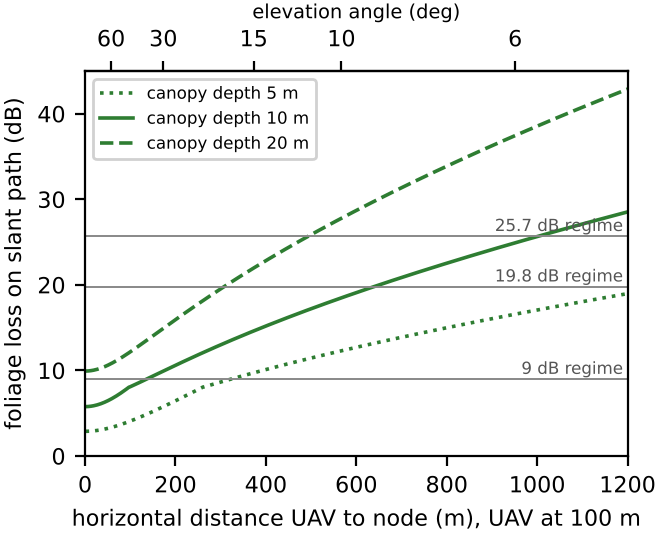
\includegraphics[width=0.92\columnwidth]{draft2-canopy-loss-labelled.png}
\caption{Weissberger foliage loss on the slant path from a UAV at 100\,m to a device under a canopy of depth 5, 10 and
20\,m, versus horizontal distance (bottom) and elevation angle (top). Horizontal lines: the constant excess losses of
the three canopy regimes.}\label{fig:canopy}
\end{figure}

\begin{figure}[t]\centering
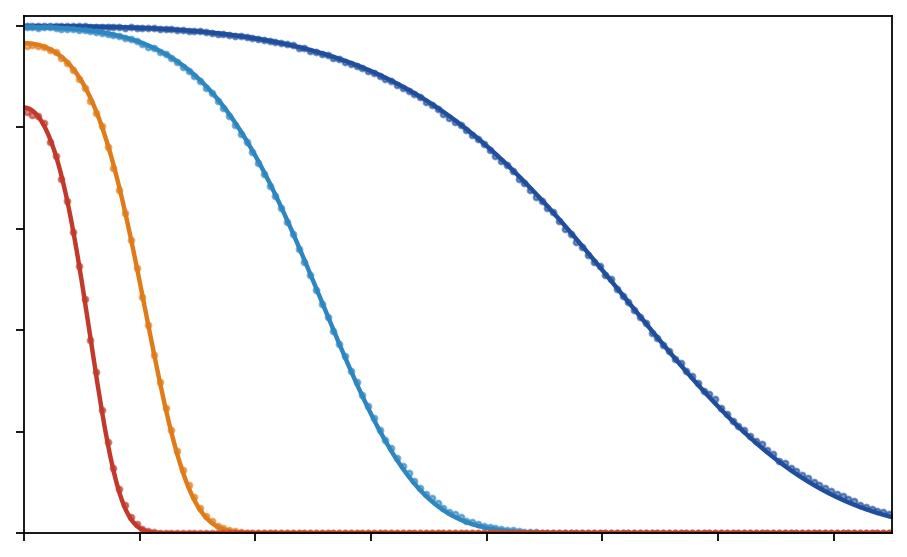
\includegraphics[width=0.86\columnwidth]{nd1-channel-p-of-d-model-vs-ns3.png}
\caption{Packet reception versus horizontal distance for the four regimes, from $R_{50}=1016$\,m (rightmost) to 99\,m.
Dots: ns-3 passes in 10\,m bins. Lines: model \eqref{eq:pd} with one common threshold. \todo{labelled version.}}
\label{fig:channel}
\end{figure}

The CL gathers what the devices of its cell hold, so the relevant event is that some device of the cell hears the
packet. For a cell $c$ with device set $U_c$ and the UAV above $x$,
\begin{equation}
P_c(x)=1-\prod_{u\in U_c}\bigl(1-p(\lVert x-u\rVert)\bigr).\label{eq:pcell}
\end{equation}
\begin{assumption}[Independent receptions]\label{as:indep}
Receptions of one packet at different devices are independent.
\end{assumption}
Assumption~\ref{as:indep} is used only in \eqref{eq:pcell}; the bounds of Section~\ref{sec:limits} need only the
marginals $P_c(x)$.

\subsection{Ground links under the canopy}\label{sec:g2g}
Ground links follow a log-distance model with exponent 3.5, log-normal shadowing ($\sigma=7.8$\,dB, drawn once per
device pair) and Rayleigh fading in 100\,ms blocks, plus a foliage excess loss $L_{\mathrm f}(d)$ for a link of length
$d$. With Weissberger's model, $L_{\mathrm f}$ is 12.6\,dB at 30\,m, 17\,dB at 50\,m and 25.6\,dB at 100\,m.
\open{a model measured for devices near the ground in forest; the exponent 3.5 and the shadowing come from an urban
street model \cite{tr38901} and the two losses may double count.} Under CSMA/CA with acknowledgements, an acknowledged hop
of a 127\,B frame occupies its medium for at least 4.8\,ms and for $\tau_f\approx5$--7\,ms in practice.

\subsection{Query, coding and completion}
The query consists of $L=12$ reference images, $Q=4041$ packets in total. The UAV repeats the query along its track;
with a rateless code a cell decodes once it holds $\lceil(1+\epsilon)Q\rceil$ distinct coded packets ($\epsilon=0.05$),
and no code decodes from fewer than $Q$. The \emph{completion time} $C_k$ of critical cell $k$ is the first time at
which its CL holds enough packets to decode the query.

\subsection{Background data}
Before any incident, every device $u$ sends a record of each person it detects to its AI node: an embedding if $u$ has
an accelerator, otherwise a crop. Let $\lambda_u$ be the resulting byte rate. The background traffic may use at most a
fraction $\bar u$ (10 or 20\,\%) of the airtime of every medium. In a forest, people are rare: most camera-trap
pictures show animals or nothing, so $\lambda_u$ is much smaller than in a city. \todo{rate of human detections per
camera trap from a published dataset; Kissling \emph{et al.} report about 40 pictures per camera per day
\cite{kissling2024}.}

\subsection{Prior, reports and verification}
The person is in cell $c^\star$, drawn from a prior $\pi=(\pi_c)_{c\in\mathcal C}$ over the incident area. We consider
two priors: a uniform prior, which assumes nothing; and a prior around the last-seen point $x_0$,
$\pi_c\propto g(\lVert c-x_0\rVert)$, where $g$ is the distribution of the distance between the last-seen point and the
find location for the subject category \cite{koester2008}. \open{which prior is the main case.} A device that saw the
person stores detections whose similarity to the query is higher than that of other persons; the score model is the
binormal model of our conference version. After completion, AI node $k$ matches and reports a score through its CH over
LoRa at time $r_k$ (one message per 40\,s under the duty cycle \cite{etsi220}). The BS updates the posterior $p_c(t)$ at
every report. Team~2 verifies one cell per visit and recognises the person if it visits $c^\star$.

\subsection{Mission time}
The mission time $T^\star$ is the time from the take-off of team~1 until team~2 confirms the person. It is random
through $\omega$ (channel, MAC, detections and scores) and through $c^\star$. We use its 0.9-quantile,
\begin{equation}
Q_{0.9}[T^\star]=\min\bigl\{\theta:\Pr\{T^\star\le\theta\}\ge0.9\bigr\},\label{eq:quantile}
\end{equation}
with the probability taken jointly over $\omega$ and $c^\star\sim\pi$. \open{joint quantile over $(\omega,c^\star)$, which
matches a prior, or the worst case $\max_{c^\star}$ of the quantile over $\omega$.} We also report $\mathbb E[T^\star]$
and the fraction of missions that confirm the person before the UAV endurance runs out.

\section{Problem Formulation}\label{sec:problem}
The ideal design chooses the AI cells, the flight of team~1, the ground transport and the policy of team~2 jointly to
minimise $Q_{0.9}[T^\star]$. We do not solve this joint problem, for two reasons. Phase~0 runs long before the incident,
when $c^\star$ and the incident area are unknown, so its decisions must serve many future missions. And the quantile of a
sum is not the sum of the quantiles, so $Q_{0.9}[T^\star]$ does not split additively across phases. We therefore state
one core problem per phase, each with its own objective, and couple them through the quantities in
Table~\ref{tab:coupling}. Each problem is written in its simplest form so that it can be recognised as a member of a
known class.

\begin{table}[t]\centering
\caption{How the three problems are coupled}\label{tab:coupling}
\footnotesize
\begin{tabular}{@{}llp{0.55\columnwidth}@{}}
\toprule
From & To & Through\\
\midrule
(P0) & (P1) & critical cells $K$; query windows $D_k$; background load, which reduces the airtime left on each medium\\
(P0) & (P2) & number of AI cells, hence false alarms and the size of the suspected set\\
(P1) & (P2) & report times $r_k$, i.e., completion plus matching plus LoRa; accuracy of the posterior\\
\bottomrule
\end{tabular}
\end{table}

\subsection{(P0) AI-cell selection}
Let $y_v\in\{0,1\}$ indicate that device $v\in V_{\mathrm p}$ is an AI node and $x_{uv}\in\{0,1\}$ that device $u$ is
assigned to $v$. The critical cells are $K(y)=\{\mathrm{cell}(v):y_v=1\}$. Let $h(u,v)$ be the number of cell hops from
$u$ to $v$, $H$ the hop limit, $\beta_u$ the memory that the records of $u$ occupy at its AI node, $B_v$ the memory of
$v$, and $a_m(u,v)$ the number of frames on medium $m$ per byte sent along the cell route from $u$ to $v$. Then
\begin{subequations}\label{eq:p0}
\begin{align}
\textbf{(P0)}\quad \min_{x,y}\ & \hat{\mathcal J}_0\bigl(K(y)\bigr)\label{eq:p0-obj}\\
\text{s.t.}\ & \textstyle\sum_{v\in V_{\mathrm p}} x_{uv}=1,\quad \forall u\in V,\label{eq:p0-assign}\\
& x_{uv}\le y_v,\quad \forall u\in V,\ v\in V_{\mathrm p},\label{eq:p0-open}\\
& h(u,v)\,x_{uv}\le H,\quad \forall u\in V,\ v\in V_{\mathrm p},\label{eq:p0-hop}\\
& \textstyle\sum_{u}\beta_u x_{uv}\le B_v\,y_v,\quad \forall v\in V_{\mathrm p},\label{eq:p0-mem}\\
& \textstyle\sum_{u,v}\lambda_u\,a_m(u,v)\,x_{uv}\,\tau_f\le\bar u,\quad \forall m\in\mathcal M.\label{eq:p0-load}
\end{align}
\end{subequations}
Constraint \eqref{eq:p0-assign} assigns every device to exactly one AI node, \eqref{eq:p0-open} only to an open one,
\eqref{eq:p0-hop} within the hop limit and \eqref{eq:p0-mem} within its memory; \eqref{eq:p0-load} keeps the background
load of every medium within the budget $\bar u$. The objective $\hat{\mathcal J}_0(K)$ is an estimate of
$Q_{0.9}[T^\star]$ for the critical set $K$, averaged over plausible incident areas. It has a phase-1 part, obtained from
a predictor of the ground completion times, and a phase-2 part that grows with $|K|$ because more AI cells produce more
false alarms. \todo{define $\hat{\mathcal J}_0$ precisely; the current solver uses the mean of the phase-1 predictor.}

In the forest, $V_{\mathrm p}$ is small: AI nodes need a clearing for their solar panel. The background load is light,
so \eqref{eq:p0-load} binds less often than in a city, and the hop and memory constraints dominate.

\emph{Class.} With \eqref{eq:p0-load} dropped and the objective replaced by the number of AI nodes $\sum_v y_v$,
(P0) is the single-source capacitated facility location problem (SSCFLP) with unit opening costs
\cite{bakker2025}; the hop limit is a coverage radius, as in the $p$-center problem. Constraint \eqref{eq:p0-load} is
where (P0) departs from facility location: the load depends on shared routes, so two distant devices still compete for
the media on their way to the same AI node.

\subsection{(P1) Delivery with fixed critical cells}
Fix $K$. Time is slotted in units of $\tau_f$ for the ground and $\Tp$ for the UAV. The decisions are:
\begin{itemize}
\item the track $q:[0,T_{\mathrm f}]\to\mathbb R^2$, with $q(0)=q(T_{\mathrm f})=\mathrm{BS}$, speed in
$[v_{\min},v_{\max}]$, curvature at most $1/\rho(v)$ and $q(t)\in F$, the set of allowed positions; the order of the
clusters is implicit in $q$;
\item the emission schedule $s$: packet $j$ is emitted at times $t_j$; the query is repeated along the track;
\item the ground plan $f^{j}_{a\to b,\tau}\in\{0,1\}$: cell $a$ sends packet $j$ to an adjacent cell $b$, or to its own
CL ($b=a$), in slot $\tau$, on medium $m(a,b)$.
\end{itemize}
Let $h^j_{c,\tau}\in\{0,1\}$ indicate that cell $c$ holds packet $j$ at slot $\tau$. Packets enter from the UAV,
$h^j_{c,0}=\mathbf 1[j\in R_c(\omega)]$ with $\Pr\{j\in R_c\}=P_c(q(t_j))$ by \eqref{eq:pcell}, and move on the ground,
$h^j_{b,\tau+1}=h^j_{b,\tau}\lor\bigvee_a f^j_{a\to b,\tau}\,\xi^j_{a\to b,\tau}(\omega)$, where $\xi$ indicates a
successful transfer. Let $D_k$ be the query window of critical cell $k$, $Q_k$ the number of packets it needs, and
$C_k=\min\{\tau:\sum_{j\in D_k}h^j_{k,\tau}\ge Q_k\}$. Then
\begin{subequations}\label{eq:p1}
\begin{align}
\textbf{(P1)}\quad \min_{q,s,f}\ & Q_{0.9}\Bigl[\max_{k\in K} C_k\Bigr]\label{eq:p1-obj}\\
\text{s.t.}\ & q \text{ Dubins-feasible},\ q(t)\in F,\ T_{\mathrm f}\le T_{\mathrm{end}},\label{eq:p1-fly}\\
& f^j_{a\to b,\tau}\le h^j_{a,\tau},\quad \forall j,a,b,\tau,\label{eq:p1-causal}\\
& \textstyle\sum_{j}\sum_{(a,b):\,m(a,b)=m} f^j_{a\to b,\tau}\le 1,\quad \forall m,\tau,\label{eq:p1-medium}\\
& e_{\mathrm{tx}}F_a+e_{\mathrm{rx}}W_a\le E_a,\quad \forall a\in\mathcal C,\label{eq:p1-energy}
\end{align}
\end{subequations}
Constraint \eqref{eq:p1-fly} is the flight envelope and endurance, \eqref{eq:p1-causal} lets a cell send only what it
holds, \eqref{eq:p1-medium} allows one transmitter per medium and slot, and \eqref{eq:p1-energy} keeps the energy of
each cell within its budget $E_a$, the sum of the budgets of its forwarding devices; here
$F_a=\sum_{j,b,\tau}f^j_{a\to b,\tau}$ is the number of frames cell $a$ sends and $W_a=t^{\mathrm{off}}_a-t^{\mathrm{on}}_a$
its wake window. \open{energy per cell or per device;
whether \eqref{eq:p1-energy} binds at realistic budgets.}

\begin{figure}[t]\centering
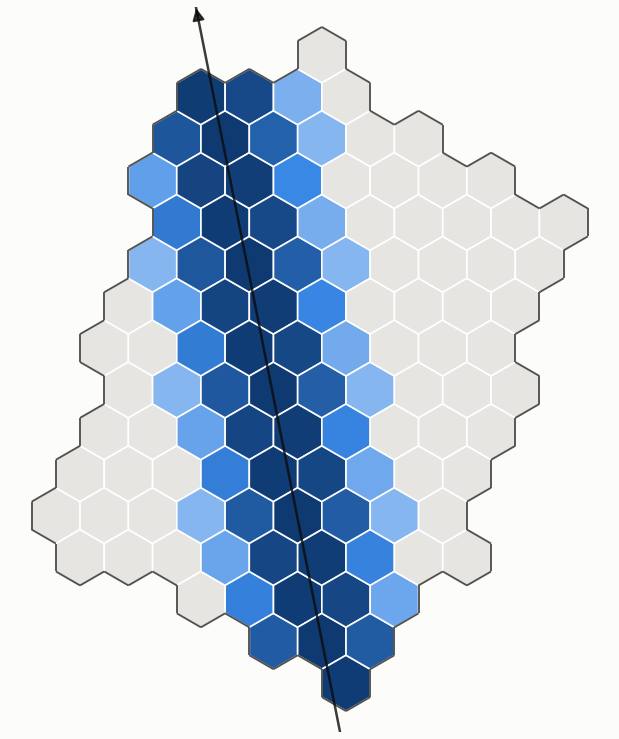
\includegraphics[width=0.62\columnwidth]{concept-river.png}
\caption{The track decides which cell holds which packets. Shade: share of the query that each cell of one cluster
receives from a single pass (darker is more). The ground plan of (P1) moves the missing shares from the dark cells under
the track to the critical cells. \todo{redraw on a forest cluster with critical cells marked.}}\label{fig:recmap}
\end{figure}

\emph{Planning information.} The reception sets $R_c(\omega)$ are known only after the pass, whereas the plan is made
before take-off. (P1) is therefore a two-stage problem. The first stage chooses $(q,s,\bar f)$ on the predicted
reception map $\hat R_c=\{j:P_c(q(t_j))\ge\vartheta\}$ (Fig.~\ref{fig:recmap}); the second stage repairs the plan on the
real reception: gathering and repair within a cell, takeover when the track deviates, and a patch for cells that remain
incomplete.

\emph{Class.} The track part is a Dubins traveling salesman problem with neighbourhoods. For fixed $q$ and reception, the
ground part is a minimum-time multicommodity broadcast schedule on a graph with unit-capacity media, in the family of
minimum broadcast time and minimum-latency broadcast scheduling \cite{you2013}. Relaxing integrality and time gives the
max-load linear programme $\min L$ subject to flow conservation from the cells under the track to the critical cells and
$\sum_{\text{flows through }m}\text{frames}\le L$ for all $m$, whence $\max_kC_k\ge\tau_fL^\star_{\mathrm{LP}}$.

\subsection{(P2) Verification}
Let $A$ be the set of suspected cells, cell $c\in A$ reported at time $r_c$, $p_c(t)$ the posterior and $d(i,j)$ the
flight time of team~2 between cells. The decisions are the take-off time $t_2$ and a policy $\mu$ that, at every
completed verification or new report, picks the next cell from the information available. If all reports were known in
advance, $\mu$ would reduce to a sequence $(c_1,c_2,\dots)$, and with $c^\star=c_{i^\star}$
\begin{equation}
T^\star=t_2+\sum_{i\le i^\star}\bigl(w_i+d(c_{i-1},c_i)+\sigma\bigr),\qquad c_0=\mathrm{BS},\label{eq:tstar}
\end{equation}
where $w_i\ge0$ is the wait if team~2 reaches $c_i$ before $r_{c_i}$. Subject to the endurance of team~2, the problem
is
\begin{equation}
\textbf{(P2)}\quad \min_{t_2,\,\mu}\ Q_{0.9}\bigl[T^\star\bigr]\quad\text{s.t. } t_2\ge\min_{c} r_c,\label{eq:p2}
\end{equation}

\emph{Class.} In the static version with the expected objective, all reports known and $t_2$ fixed, (P2) minimises
$\sum_c p_cL_c$, where $L_c$ is the time at which cell $c$ is verified: the weighted minimum latency (traveling
repairman) problem, the deterministic counterpart of the optimal searcher path problem \cite{trummel1986}. In the
static version with the 0.9-quantile, it asks for the shortest walk from the BS that visits cells of total probability
at least 0.9: a quota TSP whose quota is probability mass, with orienteering as its dual. Release times $r_c$ and
reports that arrive over time make the problem online. Without travel times, visiting cells in decreasing order of $p_c$
is optimal for the expectation (Smith's rule); the greedy policy of our conference version, which ranks cells by $p_c$
divided by travel time, is its travel-aware version.

\subsection{Complexity}
\begin{theorem}\label{thm:nphard}
The decision version of (P1) with deterministic reception, given $T$, is there a plan under which every critical cell
is complete and the UAV is back at the BS by time $T$, is NP-hard. It remains NP-hard for a single UAV of constant
speed and a ground graph without edges.
\end{theorem}
The proof \todo{Appendix A of draft v1} follows Le Ny \emph{et al.}'s reduction for the Dubins TSP \cite{leny2012}:
an instance of Exact Cover is mapped, through Papadimitriou's construction for the Euclidean TSP
\cite{papadimitriou1977} and a rescaling that absorbs both the turning-radius penalty \cite{savla2008} and the
reception radius, to an instance in which every critical cell must be overflown. The theorem locates the hardness in
the flight layer; for fixed $q$ the ground part is hard on its own, and Section~\ref{sec:limits} bounds it from below.

\begin{remark}
(P0) contains the SSCFLP, which is NP-hard \cite{bakker2025}, as the special case described above; the static
expected-value version of (P2) contains the weighted minimum latency problem, which is NP-hard even on weighted trees
\cite{sitters2002}. \todo{state both as propositions with reductions that keep the actual objectives.}
\end{remark}

\section{Limits, Algorithms and Evaluation (to be rewritten)}\label{sec:limits}\label{sec:eval}
\todo{VI Limits; VII Algorithms; VIII Evaluation on forest maps; IX Discussion (mountain parks, multiple UAVs,
density); X Conclusion. Draft v1 holds the urban-agnostic material.}

\begin{thebibliography}{99}
\bibitem{zeng2016mag} Y. Zeng, R. Zhang, and T. J. Lim, ``Wireless communications with unmanned aerial vehicles:
Opportunities and challenges,'' \emph{IEEE Commun. Mag.}, vol. 54, no. 5, pp. 36--42, May 2016.
\bibitem{mozaffari2019} M. Mozaffari, W. Saad, M. Bennis, Y.-H. Nam, and M. Debbah, ``A tutorial on UAVs for wireless
networks: Applications, challenges, and open problems,'' \emph{IEEE Commun. Surveys Tuts.}, vol. 21, no. 3,
pp. 2334--2360, 2019.
\bibitem{shen2020} Y. Shen, Y. Xiong, W. Xia, and S. Soatto, ``Towards backward-compatible representation learning,'' in
\emph{Proc. IEEE/CVF CVPR}, 2020.
\bibitem{zeng2018multicast} Y. Zeng, X. Xu, and R. Zhang, ``Trajectory design for completion time minimization in
UAV-enabled multicasting,'' \emph{IEEE Trans. Wireless Commun.}, vol. 17, no. 4, pp. 2233--2246, Apr. 2018.
\bibitem{hui2004} J. W. Hui and D. Culler, ``The dynamic behavior of a data dissemination protocol for network
programming at scale,'' in \emph{Proc. ACM SenSys}, 2004, pp. 81--94.
\bibitem{levis2004} P. Levis, N. Patel, D. Culler, and S. Shenker, ``Trickle: A self-regulating algorithm for code
propagation and maintenance in wireless sensor networks,'' in \emph{Proc. USENIX NSDI}, 2004.
\bibitem{wu2018} Q. Wu, Y. Zeng, and R. Zhang, ``Joint trajectory and communication design for multi-UAV enabled wireless
networks,'' \emph{IEEE Trans. Wireless Commun.}, vol. 17, no. 3, pp. 2109--2121, Mar. 2018.
\bibitem{liang2008} C.-J. M. Liang, R. Mus\u{a}loiu-E., and A. Terzis, ``Typhoon: A reliable data dissemination
protocol for wireless sensor networks,'' in \emph{Proc. EWSN}, LNCS 4913, 2008, pp. 268--285.
\bibitem{doddavenkatappa2013} M. Doddavenkatappa, M. C. Chan, and B. Leong, ``Splash: Fast data dissemination with
constructive interference in wireless sensor networks,'' in \emph{Proc. USENIX NSDI}, 2013, pp. 269--282.
\bibitem{du2017} W. Du, J. C. Liando, H. Zhang, and M. Li, ``Pando: Fountain-enabled fast data dissemination with
constructive interference,'' \emph{IEEE/ACM Trans. Netw.}, vol. 25, no. 2, 2017.
\bibitem{leny2012} J. Le Ny, E. Feron, and E. Frazzoli, ``On the Dubins traveling salesman problem,'' \emph{IEEE Trans.
Autom. Control}, vol. 57, no. 1, pp. 265--270, Jan. 2012.
\bibitem{isaacs2011} J. T. Isaacs, D. J. Klein, and J. P. Hespanha, ``Algorithms for the traveling salesman problem with
neighborhoods involving a Dubins vehicle,'' in \emph{Proc. American Control Conf.}, 2011, pp. 1704--1709.
\bibitem{noon1993} C. E. Noon and J. C. Bean, ``An efficient transformation of the generalized traveling salesman
problem,'' \emph{INFOR}, vol. 31, no. 1, pp. 39--44, 1993.
\bibitem{obermeyer2009} K. J. Obermeyer, ``Path planning for a UAV performing reconnaissance of static ground targets in
terrain,'' in \emph{Proc. AIAA Guidance, Navigation, and Control Conf.}, 2009.
\bibitem{nekrasov2019} M. Nekrasov, R. Allen, I. Artamonova, and E. Belding, ``Optimizing 802.15.4 outdoor IoT sensor
networks for aerial data collection,'' \emph{Sensors}, vol. 19, no. 16, 3479, 2019.
\bibitem{tr38901} 3GPP, ``Study on channel model for frequencies from 0.5 to 100 GHz,'' TR 38.901.
\bibitem{etsi220} ETSI EN 300 220-2 V3.2.1, 2018.
\bibitem{papadimitriou1977} C. H. Papadimitriou, ``The Euclidean travelling salesman problem is NP-complete,''
\emph{Theor. Comput. Sci.}, vol. 4, no. 3, pp. 237--244, 1977.
\bibitem{savla2008} K. Savla, E. Frazzoli, and F. Bullo, ``Traveling salesperson problems for the Dubins vehicle,''
\emph{IEEE Trans. Autom. Control}, vol. 53, no. 6, pp. 1378--1391, Jul. 2008.
\bibitem{heggie2009} T. W. Heggie and M. E. Amundson, ``Dead men walking: Search and rescue in US National Parks,''
\emph{Wilderness Environ. Med.}, vol. 20, no. 3, pp. 244--249, 2009. \todo{verify authors and pages}
\bibitem{koester1998} R. J. Koester, ``The lost Alzheimer's and related disorders search subject: New research and
perspectives,'' in \emph{Proc. NASAR Response 98}, 1998. \todo{verify venue}
\bibitem{koester2008} R. J. Koester, \emph{Lost Person Behavior: A Search and Rescue Guide on Where to Look for Land, Air
and Water}. Charlottesville, VA, USA: dbS Productions, 2008.
\bibitem{kissling2024} W. D. Kissling \emph{et al.}, ``Development of a cost-efficient automated wildlife camera network
in a European Natura 2000 site,'' \emph{Basic Appl. Ecol.}, vol. 79, pp. 141--152, 2024.
\bibitem{dryad} Dryad Networks, ``Silvanet wildfire sensor and mesh gateway,'' product information. [Online]. Available:
\url{https://www.dryad.net} \todo{replace by a citable source}
\bibitem{liu2013greenorbs} Y. Liu, Y. He, M. Li, J. Wang, K. Liu, and X.-Y. Li, ``Does wireless sensor network scale? A
measurement study on GreenOrbs,'' \emph{IEEE Trans. Parallel Distrib. Syst.}, vol. 24, no. 10, pp. 1983--1993, 2013.
\bibitem{zhan2018} C. Zhan, Y. Zeng, and R. Zhang, ``Energy-efficient data collection in UAV enabled wireless sensor
network,'' \emph{IEEE Wireless Commun. Lett.}, 2018. \todo{verify venue; arXiv 1708.00221}
\bibitem{nguyen2023gambac} K.-V. Nguyen, C.-H. Nguyen, T. V. Do, and C. Rotter, ``Efficient multi-UAV assisted data
gathering schemes for maximizing the operation time of wireless sensor networks in precision farming,'' \emph{IEEE Trans.
Ind. Informat.}, vol. 19, no. 12, pp. 11664--11673, 2023.
\bibitem{nguyen2021hole} K.-V. Nguyen, C.-H. Nguyen, P. L. Nguyen, T. V. Do, and I. Chlamtac, ``Energy-efficient routing
in the proximity of a complicated hole in wireless sensor networks,'' \emph{Wireless Netw.}, vol. 27, pp. 3073--3089,
2021.
\bibitem{you2013} L. You, Z. Yuan, B. Tang, and G. Chen, ``Minimum latency broadcast scheduling in single-radio
multi-channel wireless ad-hoc networks,'' arXiv:1304.5330, 2013.
\bibitem{weissberger1982} M. A. Weissberger, ``An initial critical summary of models for predicting the attenuation of
radio waves by trees,'' Electromagn. Compat. Anal. Center, Annapolis, MD, USA, Rep. ESD-TR-81-101, 1982 (DTIC
ADA118343). \todo{verify initials and report number}
\bibitem{itu833} ITU-R, ``Attenuation in vegetation,'' Recommendation P.833-10, 2021.
\bibitem{trummel1986} K. E. Trummel and J. R. Weisinger, ``The complexity of the optimal searcher path problem,''
\emph{Oper. Res.}, vol. 34, no. 2, pp. 324--327, 1986.
\bibitem{sitters2002} R. Sitters, ``The minimum latency problem is NP-hard for weighted trees,'' in \emph{Proc. IPCO},
2002, pp. 230--239.
\bibitem{hermans2019} B. Hermans, R. Leus, and J. Matuschke, ``Exact and approximation algorithms for the expanding
search problem,'' arXiv:1911.08959, 2019.
\bibitem{bakker2025} H. Bakker, G. Guastaroba, S. Nickel, and M. G. Speranza, ``The single-source capacitated facility
location problem,'' arXiv:2512.08576, 2025. \todo{verify title}
\end{thebibliography}


\end{document}
